\documentclass[
11pt,%
tightenlines,%
twoside,%
onecolumn,%
nofloats,%
nobibnotes,%
nofootinbib,%
superscriptaddress,%
noshowpacs,%
centertags]%
{revtex4}
\usepackage{ljm}
\usepackage[version=4]{mhchem}
\usepackage{stmaryrd}
\usepackage[export]{adjustbox}
\graphicspath{ {./images/} }


\begin{document}

\titlerunning{Mathematical Model of a Pulse Submerger}

\authorrunning{Kostina, Baboshin, Zhurba, Raynaud de Fitte}

\title{Mathematical Model of a Pulse Submerger and the Influence of~Manufacturing Tolerances}

\author{\firstname{Tatyana}~\surname{Kostina}}
\email[E-mail: ]{tata_sti@rambler.ru} \affiliation{ Voronezh State
Technical University, 84, 20 letiya Oktyabrya ul., 394006 Voronezh,
Russia}
\author{\firstname{Sergey}~\surname{Baboshin}}
\email[E-mail: ]{ijustbsd@gmail.com} \affiliation{ Voronezh State
University, 1 Universitetskaya pl., 394018 Voronezh, Russia}
\author{\firstname{Aleksandr}~\surname{Zhurba}}
\email[E-mail: ]{av.zhurba.93@gmail.com} \affiliation{ Voronezh
State University, 1 Universitetskaya pl., 394018 Voronezh, Russia}
\author{\firstname{Paul}~\surname{Raynaud de Fitte}}%Raynaud de Fitte P.
\email[E-mail: ]{prf@univ-rouen.fr}
\affiliation{ University of Rouen Normandy, France}

\firstcollaboration{(Submitted by A.~B.~Muravnik) }

\received{May 20, 2023, revised June 29, 2023; accepted July 10,
2023}


\begin{abstract}
This article discusses a mathematical model of the process  of
driving pile structures using an impulse driver, which is a device
based on the forces caused by the centrifugal force of imbalances.
This model is a composition of mathematical models for the operation
of an impulse driver, a model for the interaction of a pile with
soil. Also, for the first time, the issue of product operation in
the presence of belt drive defects, which can violate the ratio of
the angular velocities of the unbalances, and leads to a decrease in
the asymmetry coefficient, is considered. Gaussian white noise was
taken as a model of the belt drive errors. When setting up a
numerical experiment, the influence of instability at high speeds on
the nature of the immersion and the immersion depth was studied.
\end{abstract}

\subclass{93A30} \keywords{mathematical modeling, impulse immersion,
Maxwell--Fejer pulse, white noise} \maketitle

\section{Introduction}
There are two main methods of immersing pile structures in the soil.
This is clogging and vibration immersion. The advantage of the
second method over a hammer is to work without damaging nearby
buildings. This method of immersion is based on the effect of a
sharp decrease in the resistance to immersion of a pile element when
the latter is imparted with vibration. Such units are called
vibrators and are designed to immerse various pile elements in sandy
and clayey soils.

The mathematical model of the modified design of the vibratory pile
driver proposed in [1] posed an optimization problem for
mathematicians. Adding imbalances to the vibratory pile driver
rotating at double speeds with respect to the main shafts led to a
difference in the absolute values of the maximum and minimum of the
driving force created by the pile driver. This asymmetry effect made
it possible to create a larger positive impulse with a lower weight
of the installation. Thus, the criterion for optimization was a
parameter -- the coefficient of asymmetry, which is equal to the
ratio of the maximum to the minimum value of the function of the
driving force. The solution to the problem of constructing the
optimal impulse and a detailed description of this problem is
covered in [2] and [3]. This article describes the mathematical
impulse immersion model in Section 2.

A further development of this topic  was the application of the
impulse driver model to a mathematical model of the process of
driving a pile or sheet pile into the soil, taking into account the
rheological properties of the medium. This model is a second order
differential equation with initial conditions [4]. It takes into
account the frontal and lateral resistance of the soil to the
movement of the pile, and also includes the parameter for
controlling the operation of the impulse driver--rotation frequency
of imbalances. More details in Section 4.

In this work, for the first time, the case  is considered when the
rotation speed of shafts connected by a belt drive occurs in a white
noise field. This formulation of the problem comes from the
practical implementation of structural details and all kinds of
defects in the elements of the immersion installation. It is
important to note that the theoretical results obtained for
obtaining the optimal impulse depend on the ratio of the angular
velocities of the imbalances and, even with a slight
desynchronization, can lead to a significant deviation of the
optimal value and a change in the important parameter of the
immersion process--speed.

To study such a problem, a mathematical model  and its computer
implementation through the difference approximation in Python are
required. In the formulation of a numerical experiment, various
orders of deviations of random variables describing the defects of
the belt drive elements were considered and the dependence of the
immersion process on them was analyzed.

In the final section, graphs of the results of numerical
experiments are presented.

\section{Impulse Plunger Driving Force Model}
In the theory of immersion devices, a method of  immersion is known,
based on the effect of a sharp decrease in the resistance to
immersion of a pile element when the latter is impressed with
vibration. This effect is based on the thixotropy property of
two-phase liquids. Such units are called vibratory drivers and are
designed to immerse various pile elements in sandy and clayey soils.
The structural diagram of the vibrator is shown in Fig. 1.

\begin{center}
\includegraphics[width=0.2\linewidth]{2023_04_28_f240f32309779f8eed62g-03}
\end{center}

Figure 1. Vibrating submer. Structural diagram of the vibrator: 1 --
electric motor or hydraulic motor; 2 -- intermediate gear; 3 --
synchronizing gears; 4 -- eccentrics; 5 -- headgear; 6 -- pile

When the imbalances 4 rotate, centrifugal force  acts on their
attachment axis and the vibratory driver receives a vibrating
motion, which communicates to the pile element 6 through the
headgear 5. Eccentrics are driven into rotation by electric motor 1
(or hydraulic motor) through mechanical transmission 2 and 3 (or
directly from the motor shaft). Symmetrically located unbalance --
synchronously rotate in different directions to balance radial loads
and compensated for horizontal forces.

The mathematical model of the driving force of the vibratory driver
can be represented as
\begin{eqnarray}
F_{\text {ind }}=2 n m \omega^{2} R \cos (\omega t), \label{eq:eq_1}
\end{eqnarray}
where $F_{\text {ind }}$ is compelling force of the vibratory
driver, $n$  is the number of imbalance pairs, $m$ is imbalance
mass, $\omega$ is angular speed of rotation of imbalances (in the
figure of two), $R$ is radius of displacement of the center of mass
of the imbalance relative to the axis of rotation, $t$ is time.

A mathematical model of the formation of the driving force by  an
impulse plunger, which was proposed by V. N. Ermolenko [1], differs
from the classical vibrator in different radii of pairs of
imbalances;
\begin{eqnarray*}
\sum_{k=0}^{N} m_{k} \omega_{k}^{2} R_{k} \cos \left(\omega_{k}
t\right),
\end{eqnarray*}
where $m_{k}$ is mass of $k$th pair of imbalances, $\omega_{k}$ is
angular velocity of rotation of $k$th pair of imbalances, $R_{k}$ is
radius of unbalances.

The difference in radii also makes the angular velocity  of rotation
of the pairs of unbalances different $\omega_{k}$. In this case, the
following relation is satisfied
\begin{eqnarray}
\omega_{k}=k \omega_{0}, k=1 \ldots N. \label{eq:eq_2}
\end{eqnarray}

In an impulse immersion device, in addition  to the effect of
reducing friction by means of vibration, a key property appears,
which is the appearance of an asymmetry between useful and harmful
driving forces. We will call "useful" the driving force at the
moment when the installation plunges the pile into the ground
$\left(F_{\text {ind }}(t)>0\right)$. A "negative" driving force is
called at that moment of time when it is directed in the direction
opposite to immersion $\left(F_{\text {ind }}(t)<0\right)$. In the
case of a classic vibrator, the useful and negative driving forces
are equal in amplitude, which is clearly seen from the graph of
function (\ref{eq:eq_1}) shown in Fig. 2 (red). These amplitudes are
different for a pulse immersion (Fig. 2, green).
\begin{center}
\includegraphics[max width=0.7\textwidth]{images/Figure_1.png}
\end{center}
Figure: 2: Graph of the functions of the driving force of the
plunger with one pair of unbalances (vibrating submer, N=1, red) and
with 6 pairs of unbalances (impulse submer, N=6, green) for one time
period


The maximum useful force is the maximum of  the function $F_{\text
{ind }}(t)$, the minimum value of the function $F_{\text {ind }}(t)$
is the greatest absolute value of the negative driving force. The
absolute ratio of the maximum value of the function to the minimum
value is called the asymmetry coefficient $K_n$
%\begin{equation}\label{koef-asimmetrii}
\begin{eqnarray*}
K_n = \left| \frac{ \max\limits_{-\pi<t<\pi} F_\text{ind}(t)}{\min\limits_{-\pi<t<\pi}
F_\text{ind}(t)}\right|,
\end{eqnarray*}
where $n$ is the number of imbalance pairs in the impulse immersion
device, $t$ is the operating time in one period of the function
$F_{\text {ind }}(t)$. The problem of how to choose the radii of
imbalances to obtain the best asymmetry coefficient was solved in
[2], [3], and  [5], where the definition of the optimal impulse is
given and the theorem on the choice of the parameters of the optimal
impulse immersion is proved.

When constructing a mathematical model  of pile driving, described
in Section 4 of this work, we used the model of an optimal impulse
pile driver, specified up to a constant by the formula
\begin{eqnarray}
f_{n}(t, \lambda)=\sum_{k=1}^{n}(n-k+1) \cos (k \omega t), t \in[-\pi, \pi], \label{eq:eq_3}
\end{eqnarray}
where $\omega$ is the speed of rotation  of the first pair of
eccentrics. The function (\ref{eq:eq_3}) is called the impulse of
Maxwell--Fejer.

\section{Model of defects in belt transmission of white noise}
The theoretical impulse proposed in the previous section,  created
by the pressing device, has the highest asymmetry coefficient equal
to the number of imbalance pairs $K_{n}=\mathrm{n}$ [3]. But in
practical implementation, belt or gear drives from an electric motor
or hydraulic drive are used to impart rotation to the imbalance
shafts. A number of defects are possible in such a design. For
example, the main defects in belt drives, together with bearing
defects, are: pulley defects: misalignment, uneven wear,
misalignment with the shaft lead to a periodic change in belt
tension, which is expressed in the modulation of low-frequency
transmission vibration and friction forces in bearings with a
frequency rotation of the defective pulley. Also, the nonparallelism
of the shafts and the axial displacement of the pulleys, leading to
the occurrence of periodic shock loads on the belt (chain) with
rotation of one of the pulleys (or both), pulse modulating friction
forces in the transmission bearings and high-frequency vibration of
these bearings. In addition, the weakening of the belt tension,
leading to instability of the harmonic amplitudes with the rotation
of both shafts. Belt wear, leading to a periodic change in the
tension force, which, in turn, causes modulation of low-frequency
transmission vibration by the belt rotation frequency and its
harmonics, as well as modulation of friction forces in the
transmission bearings and high-frequency vibration of these
bearings.

All of the above is also an additional  condition for the ratio of
the rotation frequencies of the imbalance shafts (\ref{eq:eq_2}),
which leads to the following model
\begin{eqnarray*}
\omega_{k}=\omega_{k}\left(1+\delta_{k}(t)\right),
\end{eqnarray*}
where $\delta_{k}(t)$ is the error in the angular speed  of rotation
of the imbalance shaft at time $t$, caused by various defects of the
submerged units.

To select a model for such an error,  this article proposes a model
of white noise, or an additive Gaussian distribution -- a
generalized stationary random process $X(t)$ with a constant
spectral density and a normal distribution of the standard
deviation.

In a numerical experiment, we will consider  various orders of
standard deviations of the random variable $\sigma(\delta)$, which
describes the noise in the belt drive, and evaluate how much this
affects the asymmetry coefficient and the main characteristics of
the immersion process as a whole.

\section{Modeling and computer implementation of the immersion process}
In applications to construction topics, in particular  to
installations of a pile foundation, to model the processes of
driving piles, the following equation is used [7]
\begin{eqnarray}
R=F_{\text {ind }}+F_{\text {grav }}-F_{\text {lr }}-F_{\text
{drag}}, \label{eq:eq_4}
\end{eqnarray}
where $R$ is resultant force, $F_{\text {ind }}$ is the pressing
force created by the immersion unit, $F_{\text {grav }}$ is gravity,
$F_{\text {lr }}$ is lateral resistance force, $F_{\text {drag }}$
is drag force.

The solution to this equation allows to determine the  time and
depth of immersion, depending on the type of immersion installation,
pile dimensions and type of soil.

The stage when the submersible installation  pulls the pile up,
overcoming the force of gravity and soil resistance along the
lateral surface will not be considered in this work. Since, in this
case, the destruction of the pile is possible, since the concrete
pile tolerates strong compression well, but collapses when trying to
stretch. In practice, this is avoided by controlling the angular
velocity of rotation of the imbalances, preventing the device from
operating at high RPM at the beginning of the dive.

If the useful force of the immersion unit and the  force of gravity
cannot exceed the resistance of the ground, the dive will stop.
After this stage, the speed of revolutions of the imbalance shafts
increases, until the driving force becomes sufficient to continue
the pile sinking.

In what follows, we will use equation (\ref{eq:eq_4})  for the
numerical model process control.

Let $m$ denote the mass of the entire installation and let  $x(t)$
denote the depth of immersion of the pile, and $t$ is the time of
immersion of the pile. Then, $R=m a=m \ddot{x}$, where $a$ is
acceleration, $F_{\text {ind }}=m g$, where $g$ is the acceleration
due to gravity, $F_{\text {drag }}=S_{\mathrm{cs}} h_{i}(x(t),
\xi)$, where $S_{\mathrm{cs}}$ is the cross-sectional area of the
pile, $h_{i}(x(t)$, $\xi$ ) is the specific drag, $\xi$ is the
coefficient of soil working conditions under the lower end of the
pile, $F_{\mathrm{ls}}=P x(t) f_{i}(\psi)$ is the lateral resistance
force, which is the product of the pile perimeter $\mathrm{P}$, the
immersion depth $x(t)$ and the specific lateral resistance force $f
i(\psi)$, depending on the type of soil.

We will assume that at time $t=0$, the immersion depth  is 0 and the
pile is motionless. Based on this, we obtain the following
second-order differential equation with initial conditions
\begin{eqnarray}
m \ddot{x}=F_{\text {ind }}+m g+S_{\mathrm{cs}} \, h_{i}(x(t),
\xi)+P x(t) f_{i}(\psi), \label{eq:eq_5}
\end{eqnarray}
\begin{eqnarray}
x(0)=\dot{x}(0)=0. \label{eq:eq_6}
\end{eqnarray}

Solving the task (\ref{eq:eq_5}) and (\ref{eq:eq_6}) makes it
possible to determine the time and depth of immersion depending on
the characteristics of the immersion installation, the size and
weight of the pile, as well as the type of soil.

For modeling using an explicit  difference scheme. We replace
$\ddot{x}$ in equation (\ref{eq:eq_5}) by the difference
approximation
\begin{eqnarray}
\begin{gathered}
m \frac{x_{i+1}-2 x_{i}+x_{i-1}}{h^{2}}=F_{\text {ind }}+m g+S_{\mathrm{cs}}
h_{i}(x(t), \xi)+P x(t) f_{i}(\psi), \\
x_{i+1}-2 x_{i}+x_{i-1}=\frac{h^{2}}{m}\left(F_{\text {ind }}+m g+S_{\mathrm{cs}} h_{i}(x(t), \xi)+P x(t) f_{i}(\psi)\right), \\
x_{i+1}=2 x_{i}-x_{i-1}+\frac{h^{2}}{m}\left(F_{\text {ind }}+m g+S_{\mathrm{cs}} h_{i}(x(t), \xi)+P x(t) f_{i}(\psi)\right) .
\end{gathered}
\label{eq:eq_7}
\end{eqnarray}

The resulting recurrent equality allows us  to numerically calculate
the current value of the function $x$, provided $x_{0}=x_{1}=0$.

For software implementation and numerical calculation  of the depth
and time of pile loading, the Python programming language was
chosen. The program calculates the pile insertion depth using
equality (\ref{eq:eq_7}).

On the basis of this program, numerical  experiments were carried
out to simulate the processes of driving a pile by an impulse pile
driver at different values of the standard deviation of the white
noise field

\section{About the influence of external noise on the nature of~the~driving force and the immersion process}
The stop condition in the calculation was carried out  when any of
the conditions were met
\begin{enumerate}
  \item Immersion of the pile to a depth of $x(t)=4 \mathrm{~m}$. The work is done.

  \item Achieving the maximum value of the number of revolutions of
  the first pair of unbalances $\max (\omega)=3000~ \mathrm{rpm}$. However, the work has not been completed.

  \item The negative driving force will exceed the sum of the force
  of gravity and the force of lateral resistance $F_{\text {ind }}>F_{l r}+m g$,
  which can lead to the destruction of concrete piles, which are fragile to tensile deformation.

\end{enumerate}

In the article [11] we put a  random change in the angular velocity
and saw how the nature of the dive changes. This work is a direct
development of this numerical experiment. The next step was to
determine the influence of the manufacturing error for each pair of
unbalances separately and determine the error on which pair brings
the greatest reduction in the asymmetry coefficient and,
consequently, the immersion time.

The figure below shows the values of the asymmetry  coefficients for
each pair of unbalances (ordinate axis) and manufacturing errors
(abscissa axis).

\begin{center}
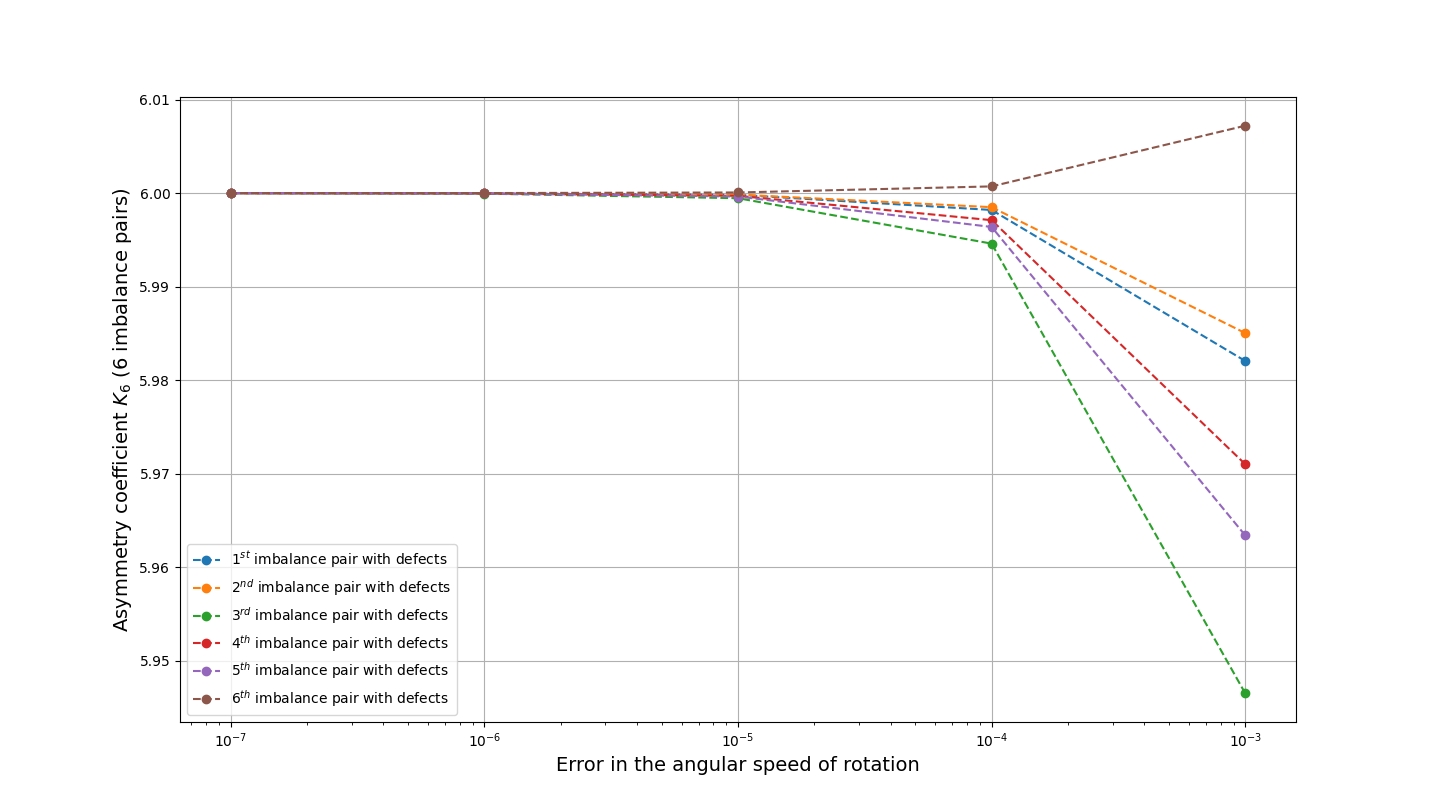
\includegraphics[max width=\textwidth]{6.png}
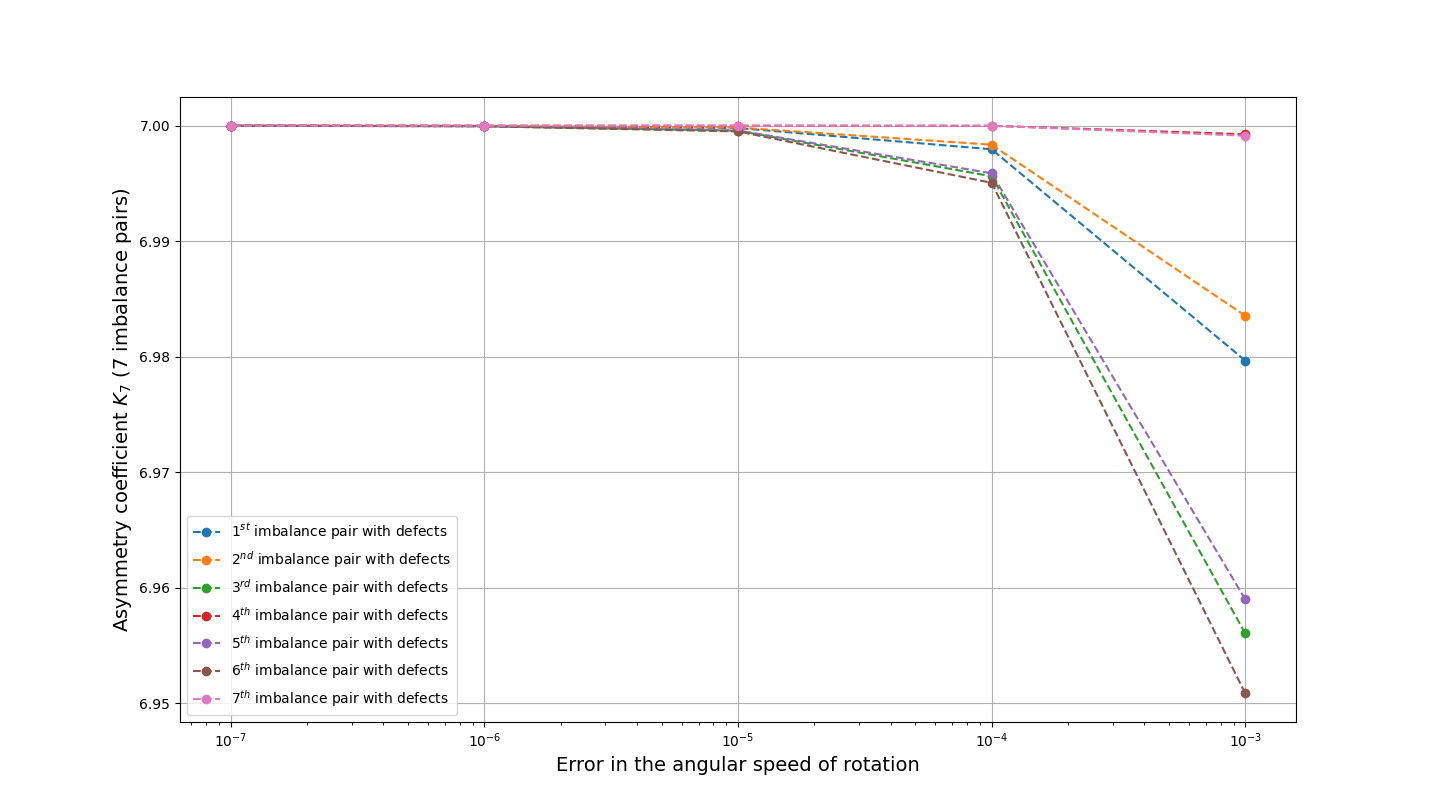
\includegraphics[max width=\textwidth]{7.png}
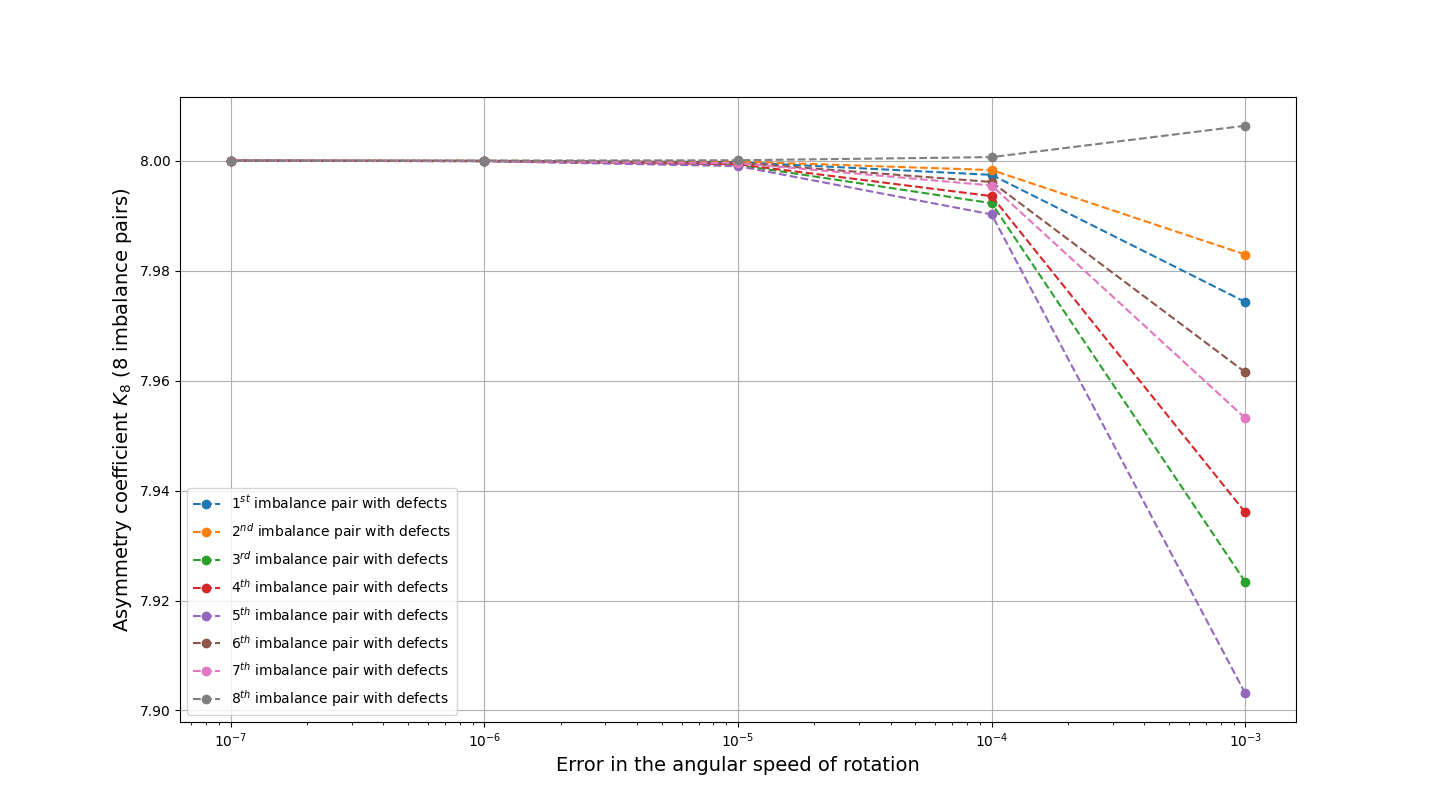
\includegraphics[max width=\textwidth]{8.png}
\end{center}


Figure: 3: Graph of the functions of the coefficients for each pair of unbalances and manufacturing errors.

%%%%%%%%%%%%%%%%%%%%%%%%%%%%%%%%%%%%%%%%%%%%%%%%%%%%%%%%%%%%%%

In the course of numerical calculations, it was  found that the
errors of the first (largest) pair of unbalances lead to the
greatest deviation of the asymmetry coefficient and thereby to a
decrease in the efficiency of the pulse submerger. This result
correlates with the result stated in [11] at the same time, it
expands and clarifies it. Since manufacturing tolerances can now be
determined for each link of the pulse submerger. The presented
formulas can be used to calculate tolerances for any devices of a
standard-sized ruler with a different number of links.

The most interesting thing is that in the case of an  even number of
unbalances and when the manufacturing error is reached on the
smallest pair above $10^{-3}$, an increase in the asymmetry
coefficient is observed. This amazing fact can be interpreted as a
transition to the next state, when the number of pairs of unbalances
is one more, which means that the asymmetry coefficient is higher.
At the same time, for an odd number of unbalances, the traditional
pattern of simply reducing the asymmetry coefficient is observed.
That is, we get an output to a more general problem when the ratio
of the angular velocities of the unbalances may not be an integer.
The study of this fact requires careful mathematical study.



{\bf Funding.} The work was supported by the RFBR grant (project
20-51-15003-NCNI\_a).


%
% The Bibliography
%

\begin{thebibliography}{99}

\bibitem{Erm1}
{V. N. Ermolenko, } "Innovative solutions for pile foundation
construction", { Stroyprofil} {\bf 6} (84), 20--22 (2010)  (In
Russian).

\bibitem{Erm2}
{ V. N. Ermolenko, I. V. Nasonov, and I. S. Surovtsev, }
"General-Purpose Identation Device", Patent RF, no. 2388868, 2009.

\bibitem{Erm3}
{V. N. Ermolenko, V. A. Kostin, D. V. Kostin, and Yu. I. Sapronov, }
"Optimization of a polyharmonic impulse", Bulletin of the South Ural
State University. Series: Mathematical Modelling, Programming and
Computer Software  {\bf 27(286)} (13), 35--44 (2012) (In Russian).


\bibitem{Kostin1}
{ V. A. Kostin, D. V. Kostin, and Yu. I. Sapronov,} "Maxwell--Fejer
Polynomials and Optimization of Polyharmonic Impulse", Doklady
Mathematics {\bf 86} (1), 512--514 (2012).

\bibitem{Kostin2}
{D. V. Kostin, T. I. Kostina, and S. D. Baboshin,} "Numerical
simulation of the pile driving process",  Modern Methods of Function
Theory and Related Problems. Materials of the International
Conference "Voronezh Winter Mathematical School", 2019, 173--174.
(In Russian).

\bibitem{Kostin3}
{ D. V. Kostin, A. S. Myznikov, A. V. Zhurba, and A. A. Utkin, }
"The program of work of the impulse plunger". The Certificate on
Official Registration of the Computer Program. No. 2020667045, 2020.

\bibitem{Kostin4}
{D. V. Kostin,} "Bifurcations of resonance oscillations and
optimization of the trigonometric impulse by the nonsymmetry
coefficient", Sbornik: Mathematics {\bf 207} (12),1709--1728 (2016).

\bibitem{Yakovleva}
{T. Yakovleva, V. Krysko-jr, and A. V. Krysko, } "Nonlinear dynamics
of the contact interaction of a three-layer plate-beam nanostructure
in a white noise field", Dynamics of Systems, Mechanisms and
Machines (6), 294--300 (2018) (In Russian).

\bibitem{Zeitlin}
{M. G. Zeitlin, V. V. Verstov, and G. G. Azbelev,} {\it "Vibration
technique and technology in pile and drilling works"}. Leningrad:
Stroyizdat, 1987. 262 p.   (In Russian).

\bibitem{Kostin5}
{D. V. Kostin, T. I. Kostina, A. V. Zhurba, and A. S. Myznikov,}
"The nonlinear mathematical model of the impulse pile driver",
Chelyabinsk Physical and Mathematical J. {\bf 6}(1),  34--41 (2021).

\bibitem{Zhurba}
A.~V.~Zhurba, S.~D.~Baboshin, and T.~I.~Kostina, P. Raynaud de Fitte
, "On the mathematical model of the process of impulsive vibration
driving process and its stability", Chelyabinsk Physical and
Mathematical J.  {\bf 7}(1), 78--88 (2022).
\end{thebibliography}

\end{document}
